\chapter{Alternative Advection Schemes}

We can generalise the results of chapters \ref{chap:advect} and \ref{chap:advectionAnalysis} to the following:
\begin{itemize}
\item First-order in space schemes are excessively diffusive
\item Second-order in space, centred, linear schemes suffer from dispersion errors which contaminate solutions with grid-scale oscillations
\item Explicit Eulerian schemes will have restricted time-steps.
\end{itemize}

These are consistent with {\bf Godunov's theorem:}\\
Linear numerical schemes for solving partial differential equations, having the property of not generating new extrema (monotone scheme), can be at most first-order accurate.

\ \\
We will therefore present some alternatives:
\begin{enumerate}
\item Semi-Lagrangian
\item Artificial diffusion to remove spurious oscillations
\item Clipping of unbounded values
\item The Finite Volume Method
\item Higher-order, upwind schemes
\item Total variation diminishing (TVD) schemes
\end{enumerate}

\clearpage
\section{Semi-Lagrangian Advection}

\subsubsubheading{CFL criterion:} The domain of dependence of the numerical
solution should include the domain of dependence of the original PDE.

\begin{itemize}
\item So any scheme for which $\phi_j^{(n+1)}$ depends only on its immediate neighbours, $\phi_{j-1}^{(n)}$,  $\phi_{j}^{(n)}$,  $\phi_{j+1}^{(n)}$ at the previous time step will have a stability restriction based on $\Delta t$. To avoid this, construct the numerical domain of dependence to contain the physical domain of dependence. 

\item Recall the linear advection equation and its analytic solution:
\end{itemize}

\begin{minipage}{0.59\linewidth}\setlength{\parskip}{6pt}
{\centering\begin{tabulary}{\linewidth}{CCC}
$\frac{\partial \phi}{\partial t} + u\frac{\partial \phi}{\partial x} = 0$, && $\phi(x,t) = \phi(x-u~t, 0)$ \\
\end{tabulary}}
\begin{itemize}
\item Semi-Lagrangian advection is defined from this:
\begin{equation*}
\phi(x_j,t_{n+1}) = \phi(x_j-u\Delta t, t_n) = \phi(x_{jd},t_n)
\end{equation*}

$x_{jd}\eq x_j\minus u\Delta t$ is the departure point of point $x_j$.

\item So interpolate $\phi$ from known points onto $x_{jd}$.

\item First find $k$ such that $x_k \le x_{jd}\le x_{k+1}$: \\
$k = \opttext{\text{int}((x_j - u\Delta t)/\Delta x) =  \text{int}(j - c)}$

\end{itemize}
\end{minipage}\hfill
\begin{minipage}{0.39\linewidth}\opttext{
\includegraphics[width=\linewidth]{figs/SL.pdf}}
\end{minipage}

\begin{itemize}
\item Interpolate from $x_{k-1}$, $x_{k}$, $x_{k+1}$, $x_{k+2}$, ... onto $x_{jd}$ (see section \ref{secn:interp}).
\item The time step is no-longer restricted by the Courant number but
for stability, a sufficiently small time step must be used so that trajectories do not cross.
\end{itemize}

{\bf Exercise} 
Find $\beta=\frac{x_{jd}-x_k}{\Delta x}$ as a function of only $j$, $k$ and $c$ given $x_j=j\Delta x$ and $c=u\Delta t/\Delta x$.\\
\opttext{$\beta=j-k-c$}

{\bf Problem}: The advected quantity is not conserved

\clearpage
\section{Artificial Diffusion to Remove Spurious Oscillations}

Numerical schemes are designed not to produce spurious oscillations. However, once a forecasting model is put together, often spurious oscillations are still generated. These can be removed by adding an aritficial diffusion term to the equations. For example, the linear advection equation with diffusion:
\begin{equation}
\frac{\partial\phi}{\partial t} + \vec{u}\dprod\nabla\phi - K\nabla^2\phi = 0
\end{equation}
or in one dimension:
\begin{equation}
\frac{\partial\phi}{\partial t} + 
\opttext{u\frac{\partial\phi}{\partial x} - K\frac{\partial^2\phi}{\partial x^2}=0}
\end{equation}
This is effective but damps oscillations at all wavelengths, not just the shortest wavelengths. And it dampens real features not just errors. $\therefore$ it is only (but frequently) used as a last resort. More scale-selective filtering can be achieved using $\nabla^4$ rather than $\nabla^2$. 

\subsubsubheading{Exercise:} Find the stability constraints on the advection-diffusion scheme:
\begin{equation}
\phi^{(n+1)}_j - \phi^{(n-1)}_j + c(\phi^{(n)}_{j+1}-\phi^{(n)}_{j-1})
- 2d(\phi^{(n-1)}_{j+1} - 2\phi^{(n-1)}_{j} + \phi^{(n-1)}_{j-1}) = 0
\end{equation}
where $c=u\Delta t/\Delta x$ and the diffusion number, $d=K\Delta t/\Delta x^2$. To simplify the algebra assume that $c=0$. (In fact, for $c\ne 0$, the stability constraint is $c^2 + 4d \le 1$.)

\clearpage
\section{Clipping of unbounded values}

If you know that your variable, $\phi$, should remain between specified limits, for example if it is concentration it should remain between zero and one or if it is density then it should be greater than zero, then values predicted outside these limits can be reset to the limits:
\begin{equation*}
\phi = \min(\max(\phi, \phi_{\min}), \phi_{\max})
\end{equation*}
Why would this be a very bad idea? \opttext{$\phi$ is no longer conserved}

\clearpage
\section{The Finite Volume Method}

The volume integrals of predicted variables (eg $\phi$) are calculated on small volumes (cells with volume $V$) by calculating the quantities entering and leaving the cell:

\begin{minipage}{0.49\linewidth}
\input{figs/fvGrid.pdf_t}
\end{minipage}
\hfill
\begin{minipage}{0.49\linewidth}\raggedright
$\frac{d}{dt}\biggl(V\phi\biggr) = \sum_{i=1}^4 f_i$

Where $f_i$ is the flux of $\phi$ through edge $i$. 

\ \\

Constant density flow is divergence free ($\nabla\cdot\mathbf{u}=0$) and so two forms of the linear advection equation are equivalent:

\ \\

\begin{tabular}{lr}
$\frac{\partial \phi}{\partial t} + \mathbf{u}\cdot\nabla\phi = 0$ & advective form\\ \ \\
$\frac{\partial \phi}{\partial t} + \nabla\cdot (\mathbf{u}~\phi) = 0$ & flux form\\
\end{tabular}
\end{minipage}

The flux (or conservative) form can be discretised using Gauss's divergence theorem:
\begin{equation*}
V~ \nabla\cdot\mathbf{u}\phi \approx \int_V \nabla\cdot\mathbf{u}\phi~ dV
    = \int_S \phi\mathbf{u}\cdot \mathbf{dS}
    \approx \sum_i f_i
\end{equation*}
where $f_i = \phi\mathbf{u}\cdot \mathbf{dS}$ is the flux over edge $i$.

\subsection{The Finite Volume Method in one dimension, for constant $u$}

To solve : $\frac{\partial \phi}{\partial t} = -\frac{\partial u\phi}{\partial x}$
\hfill
\input{figs/1dfvGrid.pdf_t}

\begin{minipage}{0.49\linewidth}\raggedright
\begin{equation*}
\frac{\partial \phi_j}{\partial t} = -\frac{f_{j+\half}-f_{j-\half}}{\Delta x}
\end{equation*}

\paragraph*{Exercise} ~Demonstrate the following:

\ \\
\begin{itemize}
\item If we choose centred in time for $\frac{\partial \phi_j}{\partial t}$ and $f_{j+\half}=\frac{u}{2}\bigl(\phi_{j+1}+\phi_j\bigr)$ we recover the CTCS finite difference scheme
\item If we choose forward in time for $\frac{\partial \phi_j}{\partial t}$ and $f_{j+\half}=u\phi_j$ we recover the FTBS finite difference scheme
\end{itemize}
\end{minipage}
%
\begin{minipage}{0.49\linewidth}
\includegraphics[width=\linewidth]{figs/mesh_face.png}
\end{minipage}

{\bf 
Using the finite volume method, we can solve equations on arbitrary meshes.
}
\clearpage
\section{High-order upwind schemes}
\subsection{QUICK (quadratic upwind)}

Using Taylor series, we can find a third-order approximation for $\phi_{j+\half}$ using $\phi_{j+1}$, $\phi_{j}$ and $\phi_{j-1}$.

\[
\phi_{j+\half} = \frac{1}{8}\bigl(3\phi_{j+1} + 6\phi_j - \phi_{j-1}\bigr)
\]
and similarly:
\[
\phi_{j-\half} = \frac{1}{8}\bigl(3\phi_{j} + 6\phi_{j-1} - \phi_{j-2}\bigr)
\]


These can be used, in conjunction with the finite volume method and forward in time stepping:
\begin{equation*}
\frac{\phi_j^{(n+1)} - \phi_j^{(n)}}{\Delta t} = -u\frac{\phi_{j+\half}^{(n)}-\phi_{j-\half}^{(n)}}{\Delta x}
\end{equation*}
to create the QUICK advection scheme. However this turns out to be unstable. It can be stabilised using Matsuno forward-backward time-stepping:
\begin{align*}
\phi_j^* &= \phi_j^{(n)} - c(\phi_{j+\half}^{(n)}-\phi_{j-\half}^{(n)})\\
\phi_j^{(n+1)} &= \phi_j^{(n)} - c(\phi_{j+\half}^*-\phi_{j-\half}^*)
\end{align*}

\clearpage
\section{Total Variation Diminishing (TVD) schemes}

\begin{itemize}
\item
Linear, second-order advection schemes produce unbounded, unrealistic, grid-scale oscillations. These can be measured by the total variation:
\begin{equation*}
TV = \sum_{j=0}^{N-1}|\phi_{j+1}-\phi_j|
\end{equation*}
\item 
A total variation diminishing (TVD) scheme has $TV^{(n+1)} \le TV^{(n)}$.
\item
First-order upwind is the only {\em linear} TVD scheme. Other TVD schemes are non-linear...
\item
We start with the linear advection equation discretised in conservative (flux) form:
\begin{equation}
\frac{\phi_j^{(n+1)} - \phi_j^{(n)}}{\Delta t} = -\frac{f_{j+\half}^{(n)} - f_{j-\half}^{(n)}}{\Delta x}.
\end{equation}
\item
Each flux, $f_{j+\half}$, is calculated as a weighted average of a high order flux ($f_H$) and a low order flux ($f_L$):
\begin{equation*}
f_{j+\half} = \Psi_{j+\half} ~f_H + (1-\Psi_{j+\half}) ~f_L
\end{equation*}
\item
Use as much of $f_H$ as possible without introducing oscillations
\item
So $\Psi$ should be close to one where the solution is smooth so that the solution is close to second-order accurate and $\Psi$ close to zero where the solution changes rapidly so as to use the upwind flux which guarantees boundedness.
\item The scheme is now non-linear since $\Psi$ depends on $\phi$.
\item
The simplest high-order flux is the centred, second-order flux ($f_H=u_{j+\half} ~\tfrac{1}{2}(\phi_{j} + \phi_{j+1})$) and the simplest low-order flux is the upwind, first-order flux ($f_L=u_{j+\half}~ \phi_j$ if $c\ge 0$ and $f_L=u_{j+\half}~ \phi_{j+1}$ if $c\le 0$).
\end{itemize}

\clearpage
TVD schemes can also be defined as a convex combination of two second-order schemes. 

Reminder: the finite volume method:

\begin{center}\begin{tabular}{lr}
$\phi_j^{(n+1)} = \phi_j^{(n)} - c(\phi_{j+\half}^{(n)}-\phi_{j-\half}^{(n)})$
& where $c=u\Delta t/\Delta x$.
\end{tabular}\end{center}

\begin{minipage}{0.49\linewidth}\centering
{\bf Lax-Wendroff}\\
$\phi_{j+\half} = \half(1+c)\phi_j + \half(1-c)\phi_{j+1}$\\
combination of centred and upwind 
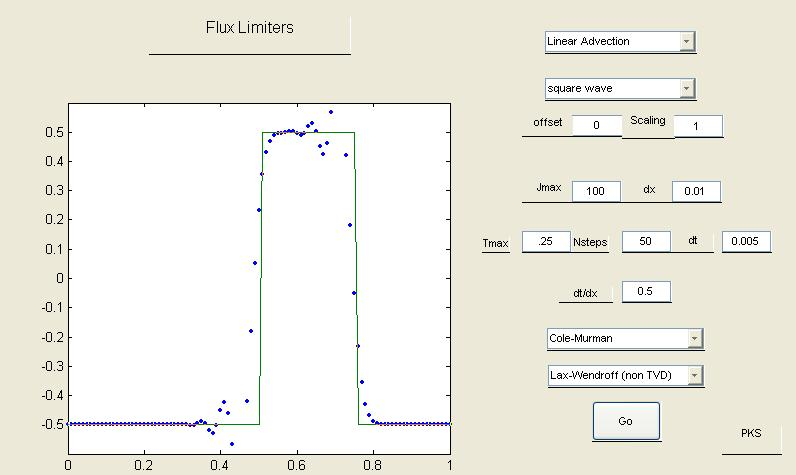
\includegraphics[width=\linewidth]{figs/lw.png}
Smooth ahead of the discontinuity
\end{minipage}
\hfill
\begin{minipage}{0.49\linewidth}\centering
{\bf Warming and Beam}\\
$\phi_{j+\half} = \half(3-c)\phi_j - \half(1-c)\phi_{j-1}$\\
combination of upwind and linear upwind
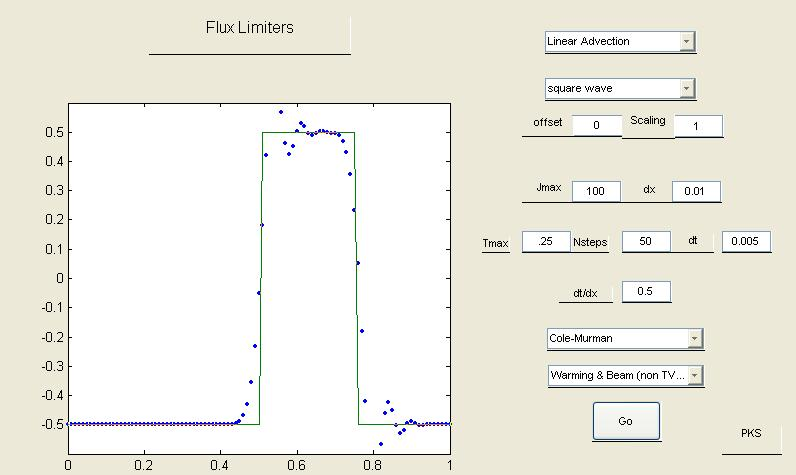
\includegraphics[width=\linewidth]{figs/wb.png}
Smooth behind the discontinuity
\end{minipage}

Lax-Wendroff is commonly used as the high-order flux for TVD schemes\\
Figures courtesy of Pete Swebey

\clearpage
\subsection{Limiter functions}

Wiggles are amplified when when one has a local minimum and more material leaves the cell on one side than enters it on the other (and conversely for a local maximum). Therefore it makes sense to let $\Psi$ be a function
of the ratio of the upwind gradient to the local gradient; for positive wind speed
\begin{equation*}
r_{j+\half} = \frac{\phi_j - \phi_{j-1}}{\phi_{j+1} - \phi_j}
\end{equation*}

\begin{minipage}[t]{0.55\linewidth}
\subsubsubheading{Exercise:}\raggedright
Mark on the graph the approximate values of $r$ at each of the cell interfaces ($j+\half$ positions).
\\
\input{figs/gradientRatio.pdf_t}
\end{minipage}
\hfill
\begin{minipage}[t]{0.44\linewidth}
\centerline{\bf How do we want $\Psi$ to vary with $r$?\\}

\begin{itemize}\raggedright
\item $r\approx 1$ (smooth monotonic): use second-order scheme
\item $r< 0$ (local extreme): use upwind scheme to avoid amplifying extreme
\item $r\approx 0$ (zero upwind gradient): use upwind scheme to avoid generating an extreme
\item $r \rightarrow\infty$ (zero local gradient): doesn't matter: upwind or second-order will produce same flux! (as long as we don't consider the upwind-upwind point for calculating $\phi_{j+\half}$ as in Warming and Beam)
\end{itemize}
\end{minipage}

\clearpage
\subsection{The Sweby Diagram}

The Sweby diagram shows the limiter function, $\Psi$, as a function of the upwind to local gradient, $r$. The shaded region indicates the region of valid second-order TVD limiter functions, assuming that Lax-Wendroff is used as the high-order flux. The two thick dashed lines indicate the ‘Superbee’ and ‘Min-mod’ limiters, representing the two extremes of the valid regions.

\begin{minipage}{0.45\linewidth}
\includegraphics[width=\linewidth]{figs/Swebey.png}
\end{minipage}
\hfill
\begin{minipage}{0.52\linewidth}\raggedright

In the shaded region the following desirable properties are satisfied:

\begin{enumerate}\raggedright
\item Total variation diminishing (removes top part of diagram)
\item Second-order except in vicinity of extrema (removes bottom part of diagram)
\item For constant gradient we should use high-order scheme: $\Psi(1) = 1$
\item Symmetric: forward and backward facing gradients should be advected at the same speed: $\Psi(r)/r = \Psi(1/r)$ (removes region above 1,1)
\end{enumerate}
\end{minipage}

\subsection{Van Leer Limiter}

A popular ``middle-of-the-road'' limiter function is due to Van Leer:
\begin{equation*}
\Psi(r) = (r+|r|)/(1+|r|)
\end{equation*}

\subsubsubheading{Task:} Sketch this on the Sweby diagram.

\subsubsubheading{Comment:} Can have $\Psi>1$! This is antidiffusion! (Can be useful or problematic )   
